\documentclass[12pt,a4paper,twoside]{report}

\title{Rewriting the Rewriter: Dynamic Optimizations of User-extensible Compiler Infrastructure}
\author{Edmund Goodman}
\date{\today}
\newcommand{\candidatenumber}{1234N}
\newcommand{\college}{Clare College}
\newcommand{\course}{Master of Philosophy in Advanced Computer Science}

% Suggested LaTeX style template for Masters project report submitted at the
% Department of Computer Science and Technology
%
% Markus Kuhn, May 2022
% (borrowing elements from an earlier template by Steven Hand)

\usepackage[pdfborder={0 0 0}]{hyperref}  % turns references into hyperlinks
\usepackage[vmargin=20mm,hmargin=25mm]{geometry}  % adjust page margins
\usepackage{graphicx} % allows inclusion of PDF, PNG and JPG images
\usepackage{parskip}  % separate paragraphs with vertical space
                      % instead of indenting their first line
\usepackage{setspace} % for \onehalfspacing
\usepackage{refcount} % for counting pages
\usepackage{upquote}  % for correct quotation marks in verbatim text

\newif\ifsubmission % Boolean flag for distinguishing submitted/final version


% ============= %
% Modifications %
% ============= %

%% Configure fonts
% \usepackage{fontspec}
% Default Serif
% \setmainfont{Linux Libertine O}[Ligatures={Common}]
\usepackage{libertine}  % Linux Libertine
% \usepackage{mathpazo}  % Palatino serif and math
% \usepackage{mathptmx}  % Times New Roman serif and math
% Sans Serif
% \usepackage{biolinum}  % Linux biolinum sans serif
% \usepackage{helvet}  % Arial (/helvetica?) sans serif
\newenvironment{defaultsffamily}{%
  \fontfamily{cmss}\selectfont
}{}
% Code
\usepackage{inconsolata}
% \setmonofont{Fira Code}[Contextuals=Alternate,Scale=MatchLowercase]

%% Extra packages
\usepackage{subcaption}
\usepackage{lastpage}       % get a reference to the last page
\usepackage{booktabs}       % professional-quality tables
\usepackage{amsfonts}       % blackboard math symbols
\usepackage{nicefrac}       % compact symbols for 1/2, etc.
\usepackage[nopatch=footnote]{microtype}      % microtypography
\usepackage{xcolor}         % colors
\usepackage{todonotes}      % todo notes
\usepackage[nottoc]{tocbibind}
\usepackage{changepage}

%% Absolute page numbers
\usepackage{zref-user}
\usepackage{zref-abspage}

%% Glossaries
\usepackage[acronym,shortcuts]{glossaries}
\makeglossaries

%% Caption configuration
\usepackage{caption}
\captionsetup{%
    labelfont=bf,%
    % textfont=it,%
    font=small,%
    skip=0pt,%
    width=0.8\textwidth%,
}
% \captionsetup{textfont=it}
% \renewcommand\fbox{\fcolorbox{white}{white}}
\captionsetup[figure]{skip=5pt}
\captionsetup[table]{skip=5pt}
% \captionsetup[listing]{skip=0pt}

%% Code highlighting
\usepackage{minted}
\setminted{%
    linenos,%
    breaklines,%
    autogobble,%
    % frame=lines,%
    % escapeinside=||,
}
% https://tex.stackexchange.com/a/53540
\newenvironment{code}{\captionsetup{type=figure,name=Listing}}{}

%% Configure urls
\usepackage{url}
% \hypersetup{
% 	colorlinks=true,
% 	linkcolor=black,
% 	urlcolor=black,
% 	citecolor=black
% }

%% Configure bibliography
\usepackage[citestyle=ieee]{biblatex}
\addbibresource{references.bib}
% Avoid overflowing URLs (https://stackoverflow.com/a/43593557)
\setcounter{biburllcpenalty}{7000}
\setcounter{biburlucpenalty}{8000}





% ======================================================================= %
% OpenCompl modifications                                                 %
% - <https://github.com/opencompl/paper-template/blob/main/tex/setup.tex> %
% - <https://github.com/opencompl/paper-template/blob/main/paper.tex>     %
% ======================================================================= %

% %%%%%%%%%%%%%%%%%%%%%%%%%%%%%%%%%%%%%%%%%%%%%%%%%%%%%%%%%%%%%%%%%%%%%%%%%%%%%%%
% % Add minted and support custom lexers
% %%%%%%%%%%%%%%%%%%%%%%%%%%%%%%%%%%%%%%%%%%%%%%%%%%%%%%%%%%%%%%%%%%%%%%%%%%%%%%%
% \usepackage{etoolbox}

% \makeatletter
% \ifcsdef{minted@optlistcl@quote}
% {
% \ifwindows
%   \renewcommand{\minted@optlistcl@quote}[2]{%
%     \ifstrempty{#2}{\detokenize{#1}}{\detokenize{#1="#2"}}}
% \else
%   \renewcommand{\minted@optlistcl@quote}[2]{%
%     \ifstrempty{#2}{\detokenize{#1}}{\detokenize{#1='#2'}}}
% \fi

% % similar to \minted@def@optcl@switch
% \newcommand{\minted@def@optcl@novalue}[2]{%
%   \define@booleankey{minted@opt@g}{#1}%
%     {\minted@addto@optlistcl{\minted@optlistcl@g}{#2}{}%
%      \@namedef{minted@opt@g:#1}{true}}
%     {\@namedef{minted@opt@g:#1}{false}}
%   \define@booleankey{minted@opt@g@i}{#1}%
%     {\minted@addto@optlistcl{\minted@optlistcl@g@i}{#2}{}%
%      \@namedef{minted@opt@g@i:#1}{true}}
%     {\@namedef{minted@opt@g@i:#1}{false}}
%   \define@booleankey{minted@opt@lang}{#1}%
%     {\minted@addto@optlistcl@lang{minted@optlistcl@lang\minted@lang}{#2}{}%
%      \@namedef{minted@opt@lang\minted@lang:#1}{true}}
%     {\@namedef{minted@opt@lang\minted@lang:#1}{false}}
%   \define@booleankey{minted@opt@lang@i}{#1}%
%     {\minted@addto@optlistcl@lang{minted@optlistcl@lang\minted@lang @i}{#2}{}%
%      \@namedef{minted@opt@lang\minted@lang @i:#1}{true}}
%     {\@namedef{minted@opt@lang\minted@lang @i:#1}{false}}
%   \define@booleankey{minted@opt@cmd}{#1}%
%       {\minted@addto@optlistcl{\minted@optlistcl@cmd}{#2}{}%
%         \@namedef{minted@opt@cmd:#1}{true}}
%       {\@namedef{minted@opt@cmd:#1}{false}}
% }
% \minted@def@optcl@novalue{customlexer}{-x}
% }
% {
% }
% \makeatother

%%%%%%%%%%%%%%%%%%%%%%%%%%%%%%%%%%%%%%%%%%%%%%%%%%%%%%%%%%%%%%%%%%%%%%%%%%%%%%%
% Base style and command for \circled to print a colored circle
%%%%%%%%%%%%%%%%%%%%%%%%%%%%%%%%%%%%%%%%%%%%%%%%%%%%%%%%%%%%%%%%%%%%%%%%%%%%%%%
% Width is assured to be the same across all characters using the typewriter font which is monospaced
% Zeroing out the inner separator removes padding between content and node (inner sep).
% Zeroing out the outer separator removes space between the node border and its anchors (e.g., east).
% Minimum size was derived on experimentation and it may need adjustment when changing font style/size.
%
% There is no guarantee for the letter ascenders/descenders to baseline when set to char.base, hence adding \strut.
% which is an invisible vertical rule with the height and depth of the parentheses ( and ).
% It ensures that the line height in a line of text is at least as large as if it contained parentheses.

\usepackage{tikz}
\usetikzlibrary{arrows}
\usetikzlibrary{shapes}

\tikzset{
  circledstyle/.style={
    shape=circle,
    #1,
    font=\tt\small,
    inner sep=0pt,
    outer sep=0pt,
    minimum size=1.2em,
    text=black
  }
}

% define a base tikz node for circled commands accepting a fill colour and the node text as arguments
\DeclareRobustCommand{\circledbase}[3][]{%
    \tikz[baseline=(char.base)]{\node[circledstyle, fill=#2] (char) {#3\strut};}%
}

% % listings don't write "Listing" in autoref without this.
% \providecommand*{\listingautorefname}{Listing}

%%%%%%%%%%%%%%%%%%%%%%%%%%%%%%%%%%%%%%%%%%%%%%%%%%%%%%%%%%%%%%%%%%%%%%%%%%%%%%%
% Add minted aliases
%%%%%%%%%%%%%%%%%%%%%%%%%%%%%%%%%%%%%%%%%%%%%%%%%%%%%%%%%%%%%%%%%%%%%%%%%%%%%%%

\usemintedstyle{colorful}

% % Newer versions of minted require the 'customlexer' argument for custom lexers
% % whereas older versions require the '-x' to be passed via the command line.
% \makeatletter
% \ifcsdef{MintedExecutable}
% {
%   % minted v3
%   \newminted[mlir]{tools/lexers/MLIRLexer.py:MLIRLexerOnlyOps}{mathescape}
%   \newminted[xdsl]{tools/lexers/MLIRLexer.py:MLIRLexer}{mathescape, style=murphy}
% }
% {
%   \ifcsdef{minted@optlistcl@quote}
%   {
%     \newminted[mlir]{tools/lexers/MLIRLexer.py:MLIRLexerOnlyOps}{customlexer, mathescape}
%     \newminted[xdsl]{tools/lexers/MLIRLexer.py:MLIRLexer}{customlexer, mathescape, style=murphy}
%   }
%   {
%     \newminted[mlir]{tools/lexers/MLIRLexer.py:MLIRLexerOnlyOps -x}{mathescape}
%     \newminted[xdsl]{tools/lexers/MLIRLexer.py:MLIRLexer -x}{mathescape, style=murphy}
%   }
% }
% \makeatother
% \newminted[mlir]{tools/lexers/MLIRLexer.py:MLIRLexerOnlyOps}{customlexer, mathescape}
% \newminted[xdsl]{tools/lexers/MLIRLexer.py:MLIRLexer}{customlexer, mathescape, style=murphy}

%%%%%%%%%%%%%%%%%%%%%%%%%%%%%%%%%%%%%%%%%%%%%%%%%%%%%%%%%%%%%%%%%%%%%%%%%%%%%%%
% Add colour scheme
%%%%%%%%%%%%%%%%%%%%%%%%%%%%%%%%%%%%%%%%%%%%%%%%%%%%%%%%%%%%%%%%%%%%%%%%%%%%%%%

% We use the following color scheme
%
% This scheme is both print-friendly and colorblind safe for
% up to four colors (including the red tones makes it not
% colorblind safe any more)
%
% https://colorbrewer2.org/#type=qualitative&scheme=Paired&n=4

\definecolor{pairedNegOneLightGray}{HTML}{cacaca}
\definecolor{pairedNegTwoDarkGray}{HTML}{827b7b}
\definecolor{pairedOneLightBlue}{HTML}{a6cee3}
\definecolor{pairedTwoDarkBlue}{HTML}{1f78b4}
\definecolor{pairedThreeLightGreen}{HTML}{b2df8a}
\definecolor{pairedFourDarkGreen}{HTML}{33a02c}
\definecolor{pairedFiveLightRed}{HTML}{fb9a99}
\definecolor{pairedSixDarkRed}{HTML}{e31a1c}


% Select which version this is:
% For the (anonymous) submission (without your name or acknowledgements)
% uncomment the following line (or let the makefile do this for you)
%\submissiontrue
% For the final version (with your name) leave the above commented.

\begin{document}

%TC:ignore
\pagenumbering{gobble}
\ifsubmission
% ================================================ %
% Submission proforma cover page for blind marking %
% ================================================ %

\begin{defaultsffamily}
\begin{titlepage}
\makeatletter

% University logo with shield hanging in left margin
\hspace*{-14mm}
\includegraphics[width=65mm]{images/logo-dcst-colour}

% submission proforma cover page for blind marking
\begin{Large}
\vspace{20mm}
Research project report title page

\vspace{35mm}
Candidate \candidatenumber

\vspace{42mm}
\textsl{``\@title''}

\end{Large}

\vspace{\fill}
\begin{center}
Submitted in partial fulfillment of the requirements for the\\
\course
\end{center}

\makeatother
\end{titlepage}
\end{defaultsffamily}
\newpage

\else
% ================== %
% Regular cover page %
% ================== %

\begin{titlepage}

\makeatletter
\begin{center}
\vspace*{\stretch{1}}
\noindent
\huge
\@title \\
\end{center}

\begin{center}
\vspace*{\stretch{1}}
\noindent
\huge
\@author \\
\Large
\college \\[24pt]

\includegraphics{images/logo-notext-colour.pdf}
\end{center}

\vspace{24pt}

\begin{center}
\vspace*{\stretch{1}}
\noindent
\large
{
    \today \\
    \vspace{0.5em}
    \it A dissertation submitted to the University of Cambridge \\
in partial fulfilment of the requirements for the degree of \\
Master of Philosophy in Advanced Computer Science
}
\end{center}

\end{titlepage}
\makeatother



% \begin{titlepage}
% \makeatletter

% % University logo with shield hanging in left margin
% \hspace*{-14mm}
\includegraphics[width=65mm]{images/logo-dcst-colour}

% % regular cover page
% \begin{center}
% \Huge
% \vspace{\fill}

% \@title
% \vspace{\fill}

% \@author
% \vspace{5mm}

% \Large
% \college
% \vspace{\fill}

% \@date
% \vspace{\fill}
% \end{center}

% \vspace{\fill}
% \begin{center}
% Submitted in partial fulfillment of the requirements for the\\
% \course
% \end{center}

% \makeatother
% \end{titlepage}



\newpage
\fi
% ================= %
% Joined cover page %
% ================= %

% \begin{sffamily}
% \begin{titlepage}
% \makeatletter

% % University logo with shield hanging in left margin
% \hspace*{-14mm}
\includegraphics[width=65mm]{images/logo-dcst-colour}

% \ifsubmission
% % submission proforma cover page for blind marking
% \begin{Large}
% \vspace{20mm}
% Research project report title page

% \vspace{35mm}
% Candidate \candidatenumber

% \vspace{42mm}
% \textsl{``\@title''}

% \end{Large}

% \else

% % regular cover page
% \begin{center}
% \Huge
% \vspace{\fill}

% \@title
% \vspace{\fill}

% \@author
% \vspace{5mm}

% \Large
% \college
% \vspace{\fill}

% \@date
% \vspace{\fill}

% \end{center}

% \fi

% \vspace{\fill}
% \begin{center}
% Submitted in partial fulfillment of the requirements for the\\
% \course
% \end{center}

% \makeatother
% \end{titlepage}
% \end{sffamily}

% \newpage
\ifsubmission
% ===================== %
% Submission cover page %
% ===================== %

\begin{defaultsffamily} % use a sans-serif font for the pro-forma cover sheet
Total page count: \pageref{LastPage}

% calculate number of pages from
% \label{firstcontentpage} to \label{lastcontentpage} inclusive
\makeatletter
\@tempcnta=\getpagerefnumber{lastcontentpage}\relax%
\advance\@tempcnta by -\getpagerefnumber{firstcontentpage}%
\advance\@tempcnta by 1%
\xdef\contentpages{\the\@tempcnta}%
\makeatother

Main chapters (excluding front-matter, references and appendix):
\contentpages~pages
(pp~\pageref{firstcontentpage}--\pageref{lastcontentpage})

Main chapters word count: 467

\vspace*{1em}
Methodology used to generate that word count:

\begin{quote}
\begin{verbatim}
$ make wordcount
gs -q -dSAFER -sDEVICE=txtwrite -o - \
   -dFirstPage=6 -dLastPage=11 report-submission.pdf | \
egrep '[A-Za-z]{3}' | wc -w
467
\end{verbatim}
\end{quote}

\end{defaultsffamily}
\vspace{\fill}
\onehalfspacing






\else
% ================== %
% Regular cover page %
% ================== %

\begin{sffamily}
Total page count: \pageref{LastPage}

% calculate number of pages from
% \label{firstcontentpage} to \label{lastcontentpage} inclusive
\makeatletter
\@tempcnta=\getpagerefnumber{lastcontentpage}\relax%
\advance\@tempcnta by -\getpagerefnumber{firstcontentpage}%
\advance\@tempcnta by 1%
\xdef\contentpages{\the\@tempcnta}%
\makeatother

Main chapters (excluding front-matter, references and appendix):
\contentpages~pages
(pp~\pageref{firstcontentpage}--\pageref{lastcontentpage})

Main chapters word count: 467

\vspace*{2em}
\begin{code}
    \begin{minted}{text}
        $ make wordcount
        gs -q -dSAFER -sDEVICE=txtwrite -o - \
           -dFirstPage=6 -dLastPage=11 report-submission.pdf | \
        egrep '[A-Za-z]{3}' | wc -w
        467
    \end{minted}
    \captionsetup{textfont=sf}
    \caption*{\textbf{Listing:} Methodology used to generate that word count.}
\end{code}



\vspace{\fill}
\onehalfspacing
\makeatletter
\textbf{\Huge Declaration}
\vspace{40pt}

I, \@author\ of \college, being a candidate for the \course, hereby
declare that this report and the work described in it are my own work,
unaided except as may be specified below, and that the report does not
contain material that has already been used to any substantial extent
for a comparable purpose.

% TODO: This doesn't show up in the submission version!!!
% Add here things like: Figure X is the work of Y, etc.
Figure \ref{fig:compilers-lagging} was created by Anton Lydike, based on a slide from Sean Silva's talk at the March 2025 Cambridge Compiler Social.

\bigskip 
\textbf{Signed:} \@author

\bigskip
\textbf{Date:} \today
\vspace{\fill}

% This dissertation is copyright \copyright \the\year{} \@author.
% \\
% All trademarks used in this dissertation are hereby acknowledged.
\makeatother

\end{sffamily}

\fi
\chapter*{Abstract}

% Write a summary of the whole thing. Make sure it fits on one page.


% == Performance profiling and optimisation of the xDSL compiler framework
% xDSL is a Python-native compiler framework, facilitating benefits such as modularity with LLVM MLIR whilst retaining simple scriptability. However, being implemented in Python comes with a performance trade-off for these benefits. We first leverage performance profiling techniques to identify bottlenecks in the xDSL project codebase, then investigate algorithmic, data structure, caching, system, and hardware-based optimisations to mitigate them. Finally, we assess the degree to which the Python's performance impact on compiler workloads can be reduced whilst retaining its benefits, strengthening the case for xDSL and its novel approach to compiler design.

% == Bringing Domain-Specific Knowledge to Dynamic Language Runtimes
% //  1. Introduction. In one sentence, what's the topic?
% The indirect nature of dynamic languages allows for changes to programs at runtime, providing greater flexibility and faster start-up times, but presents an optimization boundary for the language implementation.
% //  2. State the problem you tackle.
% API boundaries within dynamic languages may limit their dynamic nature by enforcing invariants and constraints at runtime, which could be leveraged for optimization.
% //  3. Summarize (in one sentence) why nobody else has adequately answered the research question yet.
% Previous approaches have addressed this by either tracing program execution and discovering these invariants, which incurs a runtime cost, or by using a non-dynamic DSL, which reduces flexibility.
% //  4. Explain, in one sentence, how you tackled the research question.
% We provide a user-extensible compiler from the Python AST to bytecode, allowing developers to bring their own optimization passes specific to their domain.
% //  5. In one sentence, how did you go about doing the research that follows from your big idea.
% We evaluate this by applying our performance optimizations to the xDSL compiler framework, demonstrating that it can scale to handle previously infeasible applications.
% //  6. As a single sentence, what's the key impact of your research?
% Our approach unblocks the use of Python for previously performance-bounded workloads whilst retaining its desirable dynamic properties.

% == Rewriting the Rewriter: Dynamic Optimizations of User-extensible Compiler Infrastructure
% //  1. Introduction. In one sentence, what's the topic?
MLIR is a modular compiler framework that provides core infrastructure to be leveraged and extended by users implementing their own compilers, an inherently dynamic design that bypasses its implementation language's type system as it relies on verification of invariants for user-provided abstractions.
% //  2. State the problem you tackle.
This user-extensible approach presents an inherent optimization boundary, as the data structures and transformations provided by users cannot be specialized ahead of time, meaning static ahead-of-time compilation provides fewer benefits.
% //  3. Summarize (in one sentence) why nobody else has adequately answered the research question yet.
Previous compiler frameworks accept the limitations of this optimization boundary, leveraging only the remaining optimizations offered by static ahead-of-time compilation, yet still incurring the costs of long build times and reduced flexibility, suggesting dynamic languages might be more suitable.
% //  4. Explain, in one sentence, how you tackled the research question.
We identify and mitigate the bottlenecks incurred by dynamic languages for code rewriting tasks in xDSL, a Python-native compiler framework inspired by MLIR.
% //  5. In one sentence, how did you go about doing the research that follows from your big idea.
These mitigations include adding new bytecode operations to replace bottlenecking logic, and rewriting optimisations on xDSL's own bytecode informed by domain-specific knowledge.
% //  6. As a single sentence, what's the key impact of your research?
Our research motivates the use of dynamic languages for building user-extensible compiler infrastructure, balancing performance with flexibility and fast build times.

\ifsubmission\else
% not included in submission for blind marking:

\chapter*{Acknowledgements}

This project would not have been possible without the wonderful
support of \ldots [optional]

\fi
\cleardoublepage % preserve page numbers after missing acknowledgements
\pagenumbering{roman}
\tableofcontents

\printglossary[type=\acronymtype,title={List of Abbreviations}]
\addcontentsline{toc}{chapter}{List of Abbreviations}

\newacronym{llvm}{LLVM}{Low-Level Virtual Machine}
\newacronym{mlir}{MLIR}{Multi-Level Intermediate Representation }
\newacronym{ir}{IR}{Intermediate Representation}
\newacronym{irdl}{IRDL}{Intermediate Representation Definition Language}
\newacronym{ssa}{SSA}{Static Single Assignment}

\listoffigures
\listoftables
\listoflistings
\addcontentsline{toc}{chapter}{List of Listings}
\pagenumbering{arabic}
%TC:endignore

\label{firstcontentpage} % start page count here
\chapter{Introduction}
\label{chap:introduction}

% This is the introduction where you should introduce your work. In general the thing to aim for here is to describe a little bit of the context for your work -- why did you do it (motivation), what was the hoped-for outcome (aims) -- as well as trying to give a brief overview of what you actually did.
% It's often useful to bring forward some ``highlights'' into this chapter (e.g.\ some particularly compelling results, or a particularly
% interesting finding).
% It's also traditional to give an outline of the rest of the document, although without care this can appear formulaic and tedious. Your call.




%%% "describe a little bit of the context for your work"

%% Context (~abstract sentence one: topic of compilers/MLIR)
Compilers are a critical component of computing systems, providing an abstraction for expressivity, performance, and portability from high-level programming languages to the underlying machine ISA.
Early compilers were hand-crafted, resulting in complex and language-specific implementations over their development.
The LLVM compiler framework \cite{lattnerLLVMCompilationFramework2004} addressed these problems of complexity and re-usability with a novel and language-independent \ac{ir} in \ac{ssa} form, which could be analysed and transformed by a sequence of passes.
Recently, \ac{mlir} \cite{lattnerMLIRScalingCompiler2021a}, has furthered these goals by enabling users to cheaply extend compilers with new abstractions, and automatically provides common infrastructure such as parsing and printing logic for them.




%%% "why did you do it (motivation)"

%% Context/Motivation (~abstract sentence one/two/three: extensible compiler frameworks, how this impacts performance, and that MLIR accept it)
Compiler extensibility is critical for handling the heterogenous hardware and exotic optisations of modern workloads.
However, this extensibility comes at a cost, presenting an optimisation boundary between the user and framework code. This boundary arises from the dynamic dispatch of these extensions, precluding optimisations such as ahead-of-time code motion.
This is compounded by the dynamic nature of the data structures and algorithms used by the compiler. For example, pattern rewriting in \ac{mlir} operates on a linked list representation of \ac{ssa} values -- a dynamic, pointer-chasing workload.
This further inhibits optimisations, both as a result of dynamism and not being amenable to other transformations such as vectorisation.
These factors motivate challenging the status quo of implementing user-extensible compiler frameworks in static, ahead-of-time compiled languages.






%%% "what was the hoped-for outcome (aims)"

%% Motivation/aim (~abstract sentence four: why not use dynamic languages/xDSL?)
xDSL \cite{fehrXDSLSidekickCompilation2025} is a reimplementation of \ac{mlir}'s core data structures and \ac{ir} definitions in Python, a dynamically typed, interpreted language.
xDSL's implementation in Python avoids the long build times of \ac{mlir} as a result of being interpreted. %, and its expressive syntax and minimal boilerplate allows compiler designers to focus on their task as opposed to the underlying language and framework.
In addition to this, Python's dynamic typing matches the dynamic nature of the user-extensible compiler framework workload.
However, using Python also has drawbacks, most notably in relation to runtime performance.
This work examines the performance of program optimisation through pattern rewriting in xDSL, focussing on the impact of dynamism and contrasting the current state-of-the-art, \ac{mlir}.





%%% "give a brief overview of what you actually did"


\begin{figure}
    \centering
    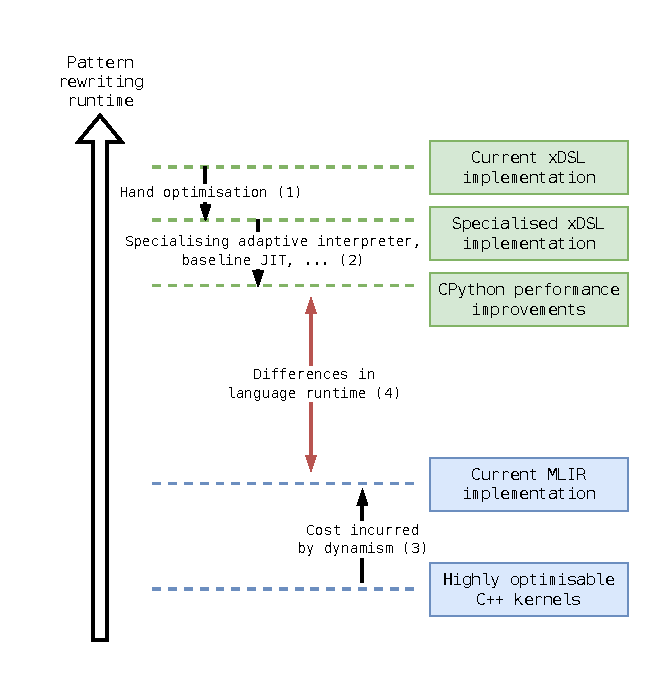
\includegraphics[width=0.7\textwidth]{images/11_introduction/narrative.drawio.pdf}
    \caption{\textit{(Sketch of figure: will be drawn properly with matplotlib and real data once finalised -- any general feedback appreciated!)} Closing the gap between xDSL (blue language runtime, orange implementation overhead) and \ac{mlir} (green) pattern rewriting performance. xDSL's performance can be improved by changes to both its implementation and language runtime. C++ has less of a performance advantage for \ac{mlir} than other workloads due to the costs associated with dynamism.}
    % TODO: Further think about this to consider making it more conceptual/hooky
    % TODO: If kept, this will have bars labelled with performance figures, but since not final have not done this yet
    \label{fig:narrative}
\end{figure}

%% Overview (~abstract sentence five, which needs re-writing: what we did part one -- specialisation and CPython stuff)
The performance of a program is constrained both by the details of its implementation and the runtime of its language.
These two properties are deeply interlinked, making them difficult to measure independently.
To disentangle them, we manually optimise and specialise xDSL's implementation for a fixed algorithm on a specific workload (Label \texttt{(1)} of \autoref{fig:narrative}), resulting in an $5.5\times$ performance uplift. % TODO: align with finalised figure when re-measured
We then confirm the performance of the specialisation is constrained only by the language runtime by examination of the dispatched bytecode of micro-benchmarks.
Following this, we quantify the impact of recent performance enhancements made to CPython for this specialised implementation (Label \texttt{(2)} of \autoref{fig:narrative}). % as an increase of $xy\%$.
This process provides an approximate best-case for the performance of pattern rewriting in xDSL, which can then be compared against \ac{mlir}.


%% Overview (~abstract sentence five, which needs re-writing: what we did part two -- custom CPython optimisations)
% Hook
% Argument
% Link


%% Overview (~abstract sentence five, which needs re-writing: what we did part three -- cost of dynamism)
A key difference between the Python and C++ runtimes is their degree of dynamism.
\ac{mlir}'s C++ runtime incurs overhead when dynamically dispatching functions (Label \texttt{(3)} of \autoref{fig:narrative}), which is worsened by prohibiting ahead-of-time performance optimisations. In contrast, almost every bytecode operation evaluated by the Python interpreter is dynamic, each incurring an overhead.
As such, we expect the difference in performance between language runtimes (Label \texttt{(4)} of \autoref{fig:narrative}) to be smaller for more dynamic workloads.
To corroborate this, we measure the difference in performance between pattern rewriting workloads using xDSL and \ac{mlir}, and assess the contribution of overheads incurred by dynamism.
Finally, we critically evaluate the degree to which this motivates the use of Python for implementing user-extensible compiler frameworks.



%% Contributions (~abstract sentence six: key impact of research)
The contributions of our work are as follows:

\begin{itemize}
    \item An examination of the best-case performance for pattern rewriting workloads in the CPython language runtime. %, including trade-offs in expressivity and the impact of performance optimisations made to the language runtime.
    \item An exploration of optimisation techniques to shrink the performance gap between dynamic and static languages for pattern rewriting workloads.
    \item A tool to examine CPython bytecode dispatch in program runs, facilitating the analysis of costs incurred by dynamism.
    \item A quantitative comparison of the performance of user-extensible compiler frameworks implemented in static and dynamic languages, focussing on the impact of dynamism.
\end{itemize}
\chapter{Background}
\label{chap:background}

% A more extensive coverage of what's required to understand your work.
% In general you should assume the reader has a good undergraduate
% degree in computer science, but is not necessarily an expert in the
% particular area you've been working on. Hence this chapter may need to
% summarize some ``text book'' material.
%
% This is not something you'd normally require in an academic paper, and
% it may not be appropriate for your particular circumstances. Indeed,
% in some cases it's possible to cover all of the ``background''
% material either in the introduction or at appropriate places in the
% rest of the dissertation.

% \section{Compilation}
% \label{sec:compilation}

% \section{LLVM and SSA}
% \label{sec:llvm-ssa}

% \section{MLIR}
% \label{sec:mlir}

% \section{IRDL and PDL}
% \label{sec:irdl}

% \section{xDSL}
% \label{sec:xdsl}

% \section{Static and dynamic languages}
% \label{sec:static-dynamic-languages}

% \section{Python internals}
% \label{sec:python-internals}

% \section{Benchmarking}
% \label{sec:benchmarking}
\chapter{Related work}
\label{chap:related-work}

% This chapter covers relevant (and typically, recent) research
% which you build upon (or improve upon). There are two complementary
% goals for this chapter:
% \begin{enumerate}
%   \item to show that you know and understand the state of the art; and
%   \item to put your work in context
% \end{enumerate}
%
% Ideally you can tackle both together by providing a critique of
% related work, and describing what is insufficient (and how you do
% better!)
%
% The related work chapter should usually come either near the front or
% near the back of the dissertation. The advantage of the former is that
% you get to build the argument for why your work is important before
% presenting your solution(s) in later chapters; the advantage of the
% latter is that don't have to forward reference to your solution too
% much. The correct choice will depend on what you're writing up, and
% your own personal preference.




\section{Static and dynamic languages}
\label{sec:static-dynamic-languages}

% Hook
% Argument
% Link

% Precisely define dynamism


% An example of where C++ dynamism presents an optimisation boundary that would otherwise be found by the compiler (and possibly that a JIT can find it?)

% Object orientated optimisations (virtual dispatch in C++/objective-C)
% Why is JS faster than Python - more constrained






\section{JIT Compilation}
\label{sec:jit-compilation}

\subsection{Copy-and-patch compilation}
\label{ssec:copy-and-patch-compilation}

\subsection{Lua JIT}
\label{ssec:lua-jit}

\subsection{GraalVM}
\label{ssec:graalvm}

\subsection{PyPI}
\label{ssec:graalvm}

\subsection{Numba, JAX, and PyTorch}
\label{ssec:number-jax-pytorch}



% \section{Python performance}
% \label{sec:python-performance}

% % \subsection{Python performance matters}
% % \label{ssec:python-performance-matters}

% Typically, we want to bind into C as much as possible -- see things like Scalene to measure this. However, for our pattern rewriting workload, this is less suitable

% \subsection{Python performance measurement}
% \label{ssec:python-perf-measurement}
% timeit/asv/pyperf and stuff maybe? Possibly not worth discussing


\subsection{Faster CPython}
\label{ssec:faster-cpython}

% Timeline

% Hook
Python is a notoriously slow language \cite{}. The Faster CPython project is an attempt to remedy this fact.
% Argument
Over the course of the recent CPython major versions, new optimisations have been incrementally added as part of this project, resulting in incremental performance gains (\autoref{tab:faster-cpython}).
% Link
This section discusses these optimisations, and their effect on CPython's performance.

% Hook
% Argument
% Link

\begin{table}[H]
  \caption{Incremental performance gains on the PyPerformance benchmark suite achieved by optimisations to the CPython interpreter.}
  \label{tab:faster-cpython}
  \centering
  \begin{tabular}{lll}
    \toprule
    \textbf{Python version} & \textbf{Optimisation over previous} & \textbf{PyPerformance result} \\
    \midrule
    CPython 3.10.17 & Baseline & $x$ \\
    CPython 3.11.12 & Specialising adaptive interpreter & $x$ \\
    CPython 3.12.10 & Comprehension inlining & $x$ \\
    CPython 3.13.3 & Version bump & $x$ \\
    CPython 3.13.3 & Enabled experimental JIT & $x$ \\
    CPython 3.14.0a7 & Version bump & $x$ \\
    CPython 3.14.0a7 & Enabled tail call interpreter & $x$ \\
    % \midrule
    % PyPy 3.11.11 & JIT compilation & $x$ \\
    \bottomrule
  \end{tabular}
\end{table}

\subsubsection{Specialising adaptive interpreter}
\label{sssec:graalvm}

\subsubsection{Comprehension inlining}
\label{sssec:graalvm}

\subsubsection{Experimental JIT compiler}
\label{sssec:graalvm}

\subsubsection{Tail call interpreter}
\label{sssec:graalvm}


\chapter{Measuring compiler framework performance}
\label{chap:measuring-compiler-performance}

%% Introduction
% Hook
In this chapter, we measure the runtime performance of two user-extensible compiler frameworks: MLIR and xDSL.
% Argument
The usefulness of these measurements are three-fold. First, we provide insight into the current relative performance of MLIR and xDSL. % interesting in its own right, and as a baseline for optimisation
Second, we identify the components of the implementation which contribute most to the overall runtime, and as such are the best targets for optimisation (\autoref{chap:specialising-optimising-pattern-rewriting}) as a corrollary of Amdahl's law \cite{amdahlValiditySingleProcessor1967}.
Finally, we isolate small, self-contained components of the implementation which are comparable between MLIR and xDSL, through which the impact of dynamism can be examined (\autoref{chap:dynamism-pattern-rewriting}).
% Link





\section{Methodology}
\label{sec:methodology}

%% Short intro
% Hook
Accurate performance measurement is a fundamental and notoriously fickle discipline in systems research. % \cite{}.
% Argument
% Link
In this section, we discuss our methodology for performance measurement, aiming to justify design decisions and facilitate reproducibility

\subsection{Experimental setup}
\label{ssec:experimental-setup}

%% Reproducibility
% Hook
The reproducibility of experiments is critical for a robust scientific methodology.
% Argument
To aid in reproducibility, we provide a description of our experimental setup (\autoref{tab:experimental-setup}).
The choice to use an AWS EC2 instance for performance measurement was partially driven by practical limitations of the resources available to the authors.
This choice incurs a cost
However, there are also commensurate benefits to this choice with respect to reproducibility. This is because researchers aiming to replicate the work can simply create their own EC2 instance with the same configuration, obviating the issue of different hardware configurations affecting performance results.
Furthermore, virtualised systems are representative of real-world workloads
In addition to this, with cloud computing becoming ubiquitous over the past decade, their is a fair body of research into reliable performance measurements on virtualised systems
% Link

\begin{table}[H]
  \caption{Summary of experimental setup configuration used for performance measurement.}
  \label{tab:experimental-setup}
  \centering
  \begin{tabular}{lll}
    \toprule
    \textbf{Configurable} & \textbf{Configuration} \\
    \midrule
    \textit{AWS instance type} & c5a.4xlarge EC2 \\
    \textit{Operating system} & Debian 24.04 (Noble) \\
    \textit{CPU name} & AMD EPYC 7R32 \\
    \textit{Logical CPU cores} & $16$ \\
    \textit{Clock frequency [MHz]} & $2799.99$ \\
    \textit{L1 Data Cache [KiB]} & $32$ \\
    \textit{L1 Instruction Cache [KiB]} & $32$ \\
    \textit{L2 Unified Cache [KiB]} & $512$ \\
    \textit{L3 Unified Cache [KiB]} & $16384$ \\
    \textit{RAM [GB]} & 16 \\
    \bottomrule
  \end{tabular}
\end{table}




\subsection{Experimental configuration}
\label{ssec:experimental-configuration}

% Hook
% Argument
% Link

\begin{table}[H]
  \caption{Summary of experimental setup configuration used for performance measurement.}
  \label{tab:experimental-configuration}
  \centering
  \begin{tabular}{lll}
    \toprule
    \textbf{Configurable} & \textbf{Configuration} \\
    \midrule
    \textit{xDSL commit SHA} & \texttt{0eda7fe} \\
    \textit{MLIR commit SHA} & \texttt{6516ae4} \\
    \midrule
    \textit{Python interpreter} & CPython 3.10.17 \\
    \textit{C++ compiler} & clang 18.1.8 \\
    \textit{CMake version} & 3.28.3 \\
    \textit{Ninja version} & 1.11.1 \\
    \bottomrule
  \end{tabular}
\end{table}



\subsection{Experimental workloads}
\label{ssec:experimental-workloads}

% Constant folding
% Hook
% Argument
% Link


\vspace{2em}

\begin{code}
    \begin{minted}{python}
import random

from xdsl.dialects.arith import AddiOp, ConstantOp
from xdsl.dialects.builtin import IntegerAttr, ModuleOp, i32
from xdsl.dialects.test import TestOp
from xdsl.ir import Operation

RANDOM_SEED = 0


def constant_folding_module(size: int) -> ModuleOp:
    """Generate a constant folding workload of a given size."""
    assert size >= 0
    random.seed(RANDOM_SEED)
    ops: list[Operation] = []
    ops.append(ConstantOp(IntegerAttr(random.randint(1, 1000), i32)))
    for i in range(1, size + 1):
        if i % 2 == 0:
            ops.append(AddiOp(ops[i - 1], ops[i - 2]))
        else:
            ops.append(ConstantOp(IntegerAttr(random.randint(1, 1000), i32)))
    ops.append(TestOp([ops[(size // 2) * 2]]))
    return ModuleOp(ops)
    \end{minted}
    \caption{.}
    \label{listing:constant-folding-workload}
\end{code}

\vspace{2em}

\begin{code}
   \centering
    \begin{minted}[fontsize=\footnotesize]{text}
"builtin.module"() ({
  %0 = "arith.constant"() {"value" = 1 : i32} : () -> i32
  %1 = "arith.constant"() {"value" = 1 : i32} : () -> i32
  %2 = "arith.addi"(%1, %0) : (i32, i32) -> i32
  %3 = "arith.constant"() {"value" = 1 : i32} : () -> i32
  %4 = "arith.addi"(%3, %2) : (i32, i32) -> i32
  %5 = "arith.constant"() {"value" = 1 : i32} : () -> i32
  %6 = "arith.addi"(%5, %4) : (i32, i32) -> i32
  %7 = "arith.constant"() {"value" = 1 : i32} : () -> i32
  %8 = "arith.addi"(%7, %6) : (i32, i32) -> i32
  %9 = "arith.constant"() {"value" = 1 : i32} : () -> i32
  %10 = "arith.addi"(%9, %8) : (i32, i32) -> i32
  %11 = "arith.constant"() {"value" = 1 : i32} : () -> i32
  %12 = "arith.addi"(%11, %10) : (i32, i32) -> i32
  %13 = "arith.constant"() {"value" = 1 : i32} : () -> i32
  %14 = "arith.addi"(%13, %12) : (i32, i32) -> i32
  %15 = "arith.constant"() {"value" = 1 : i32} : () -> i32
  %16 = "arith.addi"(%15, %14) : (i32, i32) -> i32
  %17 = "arith.constant"() {"value" = 1 : i32} : () -> i32
  %18 = "arith.addi"(%17, %16) : (i32, i32) -> i32
  %19 = "arith.constant"() {"value" = 1 : i32} : () -> i32
  %20 = "arith.addi"(%19, %18) : (i32, i32) -> i32
  "test.op"(%20) : (i32) -> ()
}) : () -> ()
    \end{minted}
    \caption{``How Slow is MLIR?'' C++ implementation.}
    \label{listing:ubenchmark-trait-checks-bench-mlir}
\end{code}



\subsection{Procedure and infrastructure}
\label{ssec:procedure-infrastructure}

% Steps actually taken

% Stuff we built

%% Corrollary benefits
% Hook
In addition to their usefulness for understanding and optimising compiler performance, these benchmarks provide an opportunity to augment the development process of the xDSL project.
% Argument
Benchmarks can be used to characterise the performance impact of changes to the xDSL codebase, making it easier to avoid unnecessary performance regression.
As such, we provide a command line interface for developers to run the benchmarks, with further functionality which supports a variety of profiling tools.
Furthermore, our benchmarks are constructed to interface with air-speed velocity \cite{michaeldroettboomAirspeedvelocityAsv2025}, a tool which runs benchmarks across repository commits. This information is tracked on the xDSL website \url{https://xdsl.dev/xdsl-bench/}, providing a dashboard for the performance characteristics of xDSL over time.
% Link


















\section{End-to-end benchmarks}

%% Introduction, goals
% Hook
The simplest metric for the performance of a system is its overall runtime.
% Argument
% Link

%% How is MLIR/xDSL split up into pipeline phases
% Hook
One of LLVM's key insights was that compilation can be split into a sequence of discrete steps, avoiding the complex control logic of previous state-of-the-art compilers.
% Argument
As such, compilers having LLVM's pedigree, such as MLIR and xDSL, can be modelled as a pipeline -- parsing the input, applying optimisation transformations, and generating a lowered output (\autoref{fig:compiler-phases}).
This allows us to break down end-to-end benchmarks into components of finer granularity for free.
% Link

%% Figure: pipeline phases

\begin{figure}
    \centering
    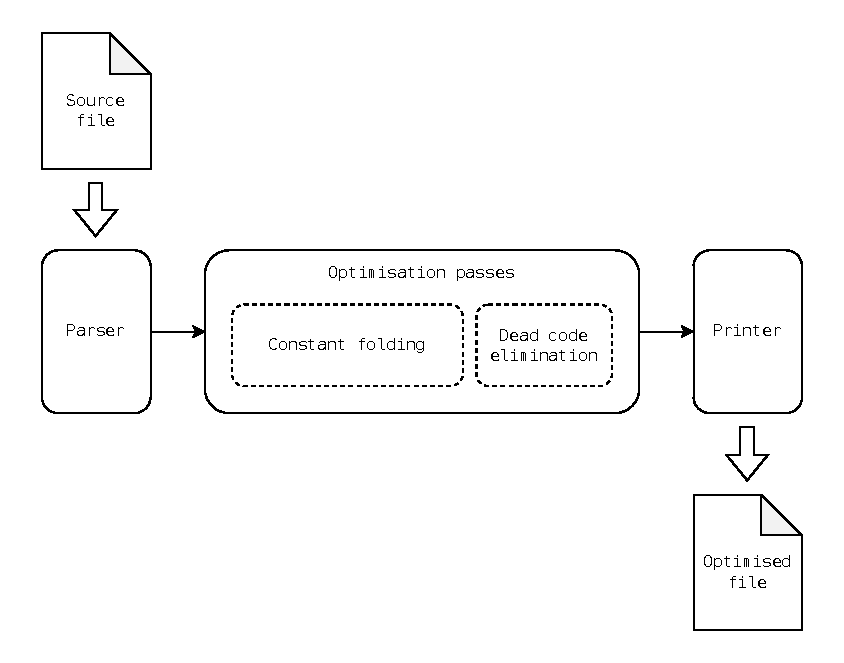
\includegraphics[width=0.75\textwidth]{images/14_measuring_compiler_performance/compiler_phases.drawio.pdf}
    \caption{.}
    % TODO: Does this add value? Could the whole thing be wrapped in an outer box to better communicate the point?
    \label{fig:compiler-phases}
\end{figure}

%% Performance results
% Hook
% Argument
% Link

% Figure: relative performance bar chart
%% Constant folding example. Short but complex example with lots of rewrites?

%% Why pick pattern rewriting?
% Hook
% Argument
% Link







\section{Pattern rewriting}

%% Introduction
% Hook
Having selected pattern rewriting as the compilation phase to examine in detail, we can modify our benchmarks to drive only


% Figure: MLIR vs xDSL across workloads?

% Figure: Trace of MLIR and xDSL overall?








\section{Micro-benchmarks}
\label{sec:ubenchmark}

% Hook
Micro-benchmarking refers measuring the performance of fast, granular, and isolated segments of code.
% Argument
The term was coined by Saavedra et al. in their 1995 paper \cite{saavedraPerformanceCharacterizationOptimizing1995} ``Performance Characterization of Optimizing Compilers''. As such, we are in good company in our application of micro-benchmarking approaches to this problem domain.
Micro-benchmarks have many desirable properties. Since they run quickly, they can cheaply be repeated for statistical confidence.
Furthermore, their fine granularity makes them tractable to reason about -- providing useful information to optimise the component of the system they measure.
However, a key difficulty of micro-benchmarking is ensuring alignment with overall system performance. For example, the selection of code paths to micro-benchmark may introduce bias, making them less representative of the overall system. In addition to this, their performance may be inflated as a consequence of warmed caches and JIT optimisations across repeats, which would not occur during normal operation.
% Link
As such, micro-benchmarking is a useful tool for deeply understanding the performance of software, but must be used carefully to ensure the validity of its results.

% Hook
As discussed in our related work (Section \ref{sec:perf-user-extensible-frameworks}), Amini and Nui's talk ``How Slow is MLIR'' \cite{aminiHowSlowMLIR2024} discusses a set of micro-benchmarks for key operations in the MLIR compiler, such as traversing the IR and creating operations.
% Argument
These micro-benchmarks were used to inform the optimisation of MLIR's data structures and for comparison with traditional LLVM-based compilers. The implementation of the micro-benchmarks allude to an underlying design goal in MLIR by their measurement of asymptotic scaling properties\footnote{\url{https://github.com/joker-eph/llvm-project/blob/6773f827b9ee8055063fcf6b2c6fcdc7f4f579d2/mlir/unittests/Benchmarks/Cloning.cpp\#L66}}. This design goal is asymptotically optimal performance for its underlying data structures. However, data structures with these characteristics often incur constant-time penalties.
This causes overhead for small workloads, where, unlike the asymptotic case, the cost is not amortised. As such, micro-benchmarks may not be representative of the system's overall performance, revealing possibility for the optimisation of code co-designed using them.
Despite this, they can still provide useful insight into MLIR's performance characteristics.
% Link
We implement micro-benchmark workloads for the xDSL equivalent to those for MLIR presented in the keynote, and compare the results of these benchmarks between the two implementations, giving insights into their relative performance.
% We further leverage profiling tools to examine the execution of the two implementations. This allows us to distinguish the cost incurred by the language runtime from the cost incurred by the algorithmic approach of the implementation.

\subsection{Implementation}
\label{ssec:ubenchmark-implementation}

%% Finding and building the MLIR microbenchmarks
% Hook
Unfortunately, the implementation and build instructions for the ``How Slow is MLIR?'' micro-benchmarks were not published with the talk.
% Argument (too informal?)
However, their source code can be found on a branch of the presenter's fork of LLVM\footnote{\url{https://github.com/joker-eph/llvm-project/tree/benchmarks}}. We provide a copy of this source code and instructions for running the benchmarks\footnote{\url{https://github.com/EdmundGoodman/llvm-project-benchmarks}} to enhance the replicability of our results and facilitate further performance experiments.
% Link
This source code can then be used to construct comparable micro-benchmarks in Python.

% Design of our microbenchmarks
% Hook
A key design goal of our micro-benchmarks for xDSL is parity with those provided for MLIR, ensuring the validity their direct comparison.
% Argument
As such, their implementation was derived from the MLIR benchmarks, matching test data and function invocations as closely as possible.
% Link3
In the following sections, we discuss the implementations of a number of micro-benchmarks, facilitating discussion of the insights they give into compiler performance across implementations and language runtimes in later chapters.


\subsection{Operation trait checks}
\label{ssec:ubenchmark-trait-checks}

% Hook
MLIR and xDSL both provide methods to check whether operations have traits.
% Argument
These methods are used very frequently in common tasks. For example, when pattern rewriting over a block of IR, the traits of the block's constituent operations are often used by the matching engine to identify valid rewrites.

% There are two factors which contribute to this slow-down. The first is the inherent overhead incurred by the interpreter loop and data structures in Python's dynamic language runtime. The second is differences in implementation between xDSL and MLIR.
% % Link
% Examining this micro-benchmark in detail allows us to decouple the performance contributions of the implementation and language runtime, and provides insight into the impact of dynamism on user-extensible compiler framework workloads.

\begin{figure}[H]
    \centering
    \begin{subfigure}[b]{0.45\textwidth}
       \centering
        \begin{minted}[fontsize=\footnotesize]{c++}
            // Setup
            Operation op = b.create<OpWithRegion>(
                unknownLoc
            );

            // Benchmark
            bool hasTrait = op->hasTrait<
                OpTrait::SingleBlock
            >();
        \end{minted}
        \caption{``How Slow is MLIR?'' C++ implementation.}
        \label{listing:ubenchmark-trait-checks-bench-mlir}
    \end{subfigure}
    \hfill
    \begin{subfigure}[b]{0.45\textwidth}
        \centering
        \begin{minted}[breakanywhere,fontsize=\footnotesize]{python}
            # Setup
            op = OpWithRegion()

            # Benchmark
            has_trait = op.has_trait(SingleBlock)
        \end{minted}
        \footnotesize\vspace{2em}
        \caption{xDSL Python implementation.}
        \label{listing:ubenchmark-trait-checks-bench-xdsl}
    \end{subfigure}
    \vspace{1em}
    \captionsetup{name=Listing}
    \caption{Micro-benchmark implementations for methods checking an operation has a trait.}
    \label{listing:ubenchmark-trait-checks-bench}
\end{figure}

Micro-benchmarks of checking traits for both implementations (Listing \ref{listing:ubenchmark-trait-checks-bench}) show a slow-down of approximately $130\times$ from MLIR to xDSL (\autoref{tab:ubenchmark-trait-checks}).

\begin{table}[H]
  \caption{Trait checks in xDSL are approximately $130\times$ slower than in MLIR in the asymptotic case.} %, repeated ten times over $32768$ operations. Methodology is discussed in detail in Appendix \ref{} to facilitate replicability.}
  \label{tab:ubenchmark-trait-checks}
  \centering
  \begin{tabular}{cc}
    \toprule
    \textbf{MLIR [ns]} & \textbf{xDSL [ns]}\\
    \midrule
    $3.89 \pm 0.01$ & $504 \pm 76$ \\
    \bottomrule
  \end{tabular}
\end{table}


% % Hook
% The trait checking micro-benchmark yields two key insights.
% % Argument
% The first is that the original implementation of xDSL makes significant tradeoffs of performance for expressivity. By eliminating these tradeoffs, we reveal the Python language runtime incurs a $16\times$ overhead with respect to C++, as a result of the complexity of its evaluation loop.
% The second is that whilst C++ can efficiently represent dynamic functionality, albeit at the cost of implementation complexity, dynamism incurs the cost of obscuring other optimisations that would further widen the performance gap between Python and C++.
% % Link
% However, whilst trait checking is a frequent operation, it alone is not representative of the overall performance of compiler frameworks. As such, further micro-benchmarks and examining representative workloads is required.


\subsection{Operation instantiation}

\subsection{Summary of micro-benchmarks}

% Hook
In addition to the above micro-benchmarks which we examine in detail, we further provide a wider suite of micro-benchmarks discussed in lesser detail for brevity. % The implementations of all xDSL micro-benchmarks are provided in the Appendix (\autoref{}).
% Argument
This suite implements many of the remaining equivalent micro-benchmarks from ``How Slow is MLIR'' (\autoref{tab:ubenchmark-remaining-mlir}).
From these, we can see the trend of a slow-down in the order of $xy\times$ holds

\begin{table}[H]
  \caption{.}
  \label{tab:ubenchmark-remaining-mlir}
  \centering
  \begin{tabular}{ccc}
    \toprule
    \textbf{Benchmark name} & \textbf{MLIR [ns]} & \textbf{xDSL [ns]}\\
    \midrule
    Trait checks & $3.89 \pm 0.01$ & $504 \pm 76$ \\
    ... & ... & ... \\
    \bottomrule
  \end{tabular}
\end{table}


% Hook
In addition to the remaining ``How Slow is MLIR?'' micro-benchmarks, the suite provides further xDSL-only micro-benchmarks sampled from atomic functions invoked by pattern rewriting workloads. % (\autoref{tab:ubenchmark-xdsl-regression}).
% Argument
These have two-fold use: triaging functions to optimise by longest runtime following Amdhal's law \cite{amdahlValiditySingleProcessor1967}; and serving as a metric of performance to ensure optimisations don't inadvertently introduce regressions.
% Link

% Do a bar chart instead of a table!!!!
% \begin{table}[H]
%   \caption{.}
%   \label{tab:ubenchmark-xdsl-regression}
%   \centering
%   \begin{tabular}{ccc}
%     \toprule
%     \textbf{Benchmark name} & \textbf{xDSL [ns]}\\
%     \midrule
%     Trait checks & $504 \pm 76$ \\
%     ... & ... & ... \\
%     \bottomrule
%   \end{tabular}
% \end{table}


\chapter{Measuring compiler framework performance}
\label{chap:measuring-compiler-performance}


% Intro

% End-to-end/pipeline-phase-wise performance of xDSL as it stands
% --> Why we pick pattern rewriting to focus on
\subsection{Compiler pipeline phases}

\subsection{Micro-benchmarks}
% Micro-benchmarks, but drop out most of the analysis
\subsection{Operation trait checks}
\subsection{Operation instantiation}

\subsection{Pattern rewriting}





\chapter{Profiling Python bytecode} % for fun and profit


\chapter{Specialising and optimising xDSL pattern rewriting}

\subsection{Constant folding workload}

\subsection{Operation trait checks}

\subsection{Operation instantiation}





\chapter{Impact of CPython performance enhancements on xDSL pattern rewriting}

\subsection{Specialising adaptive interpreter}

\subsection{JIT compilation}

\subsection{Tail call interpreter}




\chapter{Quantifying the performance impact of dynamism on C++}





\chapter{Examining the impact of dynamism on pattern rewriting in static and dynamic languages}




% \chapter{Ideally final optimisation stuff}



\chapter{Evaluation}

For any practical projects, you should almost certainly have some kind
of evaluation, and it's often useful to separate this out into its own
chapter.
\chapter{Summary and conclusions}

As you might imagine: summarizes the dissertation, and draws any
conclusions. Depending on the length of your work, and how well you
write, you may not need a summary here.

You will generally want to draw some conclusions, and point to
potential future work.
\label{lastcontentpage} % end page count here

%TC:ignore
\nocite{*}
\printbibliography[heading=bibintoc]

% \begin{thebibliography}{6} % <- adjust the number of items you have

% \bibitem{Lamport94}Leslie Lamport: \LaTeX\ -- A document preparation
% system : User's guide and reference manual. Addison-Wesley, 1994.

% \bibitem{Companion} Frank Mittelbach, Michael Goossens: The \LaTeX\
% Companion. Second edition, Addison Wesley, 2004.

% \bibitem{Knuth86} Donald E. Knuth: The \TeX book. Ad\-dison-Wesley,
%   1986.

% \bibitem{SW00} William Strunk, E.B. White, Roger Angell: The Elements
% of Style. 4th edition, Longman, 2000.

% \bibitem{Dup98} Lyn Dupre: BUGS in Writing: A guide to debugging your
% prose. 2nd edition, Addison Wesley, 1998.

% \bibitem{Zob04} Justin Zobel: Writing for Computer Science. Springer,
% 2004.

% \bibitem{Kuhn} Markus Kuhn: \LaTeX. CST Part II lecture.\\
% \url{https://www.cl.cam.ac.uk/teaching/current/TeX+Julia/materials.html}

% \end{thebibliography}
\appendix


\chapter{MLIR benchmark results}
\label{chap:mlir-benchmark-results}

\section{Pipeline phase micro-benchmark results}
% Commands to run
% Table of results

\section{How Slow is MLIR micro-benchmark results}
% Commands to run
% Table of results


\chapter{xDSL benchmark results}
\label{chap:mlir-benchmark-results}

\section{Pipeline phase micro-benchmark results}
% Commands to run
% Table of results

\section{Micro-benchmark results}
% Commands to run
% Table of results




\chapter{Bytecode profiles}
\label{chap:bytecode-profiles}

\begin{code}
    \begin{minted}[fontsize=\footnotesize]{text}
//// Trace of `has_trait_function` :

// ====== trace:403 `has_trait_function` =======                                == 61.537us
// >>> assert OP_WITH_REGION.has_trait(                                         ## 5.624us
404         2   LOAD_GLOBAL          0   (OP_WITH_REGION)                       // 1.250us
404         12  LOAD_ATTR            3   (NULL|self + has_trait)                // 583.008ns
// >>> Trait0                                                                   ## 4.500us
405         32  LOAD_GLOBAL          4   (Trait0)                               // 500.004ns
// >>> assert OP_WITH_REGION.has_trait(                                         ## 4.000us
404         42  CALL                 1   ()                                     // 291.970ns

    // ====== core:1164 `Operation.has_trait` ======                            == 45.370us
    // >>> from xdsl.dialects.builtin import UnregisteredOp                     ## 8.707us
    1176         2   LOAD_CONST           1   (0)                               // 500.004ns
    1176         4   LOAD_CONST           2   (('UnregisteredOp',))             // 333.006ns
    1176         6   IMPORT_NAME          0   (xdsl.dialects.builtin)           // 250.002ns
    1176         8   IMPORT_FROM          1   (UnregisteredOp)                  // 3.166us
    1176         10  STORE_FAST           3   (UnregisteredOp)                  // 458.967ns
    1176         12  POP_TOP                  ()                                // 208.034ns
    // >>> if issubclass(cls, UnregisteredOp):                                  ## 5.834us
    1178         14  LOAD_GLOBAL          5   (NULL + issubclass)               // 291.970ns
    1178         24  LOAD_FAST            0   (cls)                             // 250.002ns
    1178         26  LOAD_FAST            3   (UnregisteredOp)                  // 1.000us
    1178         28  CALL                 2   ()                                // 250.002ns

        //  <frozen abc>:121 `ABCMeta.__subclasscheck__`                        == 4.499us
        // >>> <source not available>                                           ## 2.750us
        123         2   LOAD_GLOBAL          1   (NULL + _abc_subclasscheck)    // 374.974ns
        123         12  LOAD_FAST            0   (cls)                          // 375.032ns
        123         14  LOAD_FAST            1   (subclass)                     // 209.024ns
        123         16  CALL                 2   ()                             // 250.002ns
        123         24  RETURN_VALUE             ()                             // 1.250us
        // =============================================

    1178         36  POP_JUMP_IF_FALSE    2   (to 42)                           // 459.026ns
    // >>> return cls.get_trait(trait) is not None                              ## 5.955us
    1181     >>  42  LOAD_FAST            0   (cls)                             // 291.038ns
    1181         44  LOAD_ATTR            7   (NULL|self + get_trait)           // 290.980ns
    1181         64  LOAD_FAST            1   (trait)                           // 790.984ns
    1181         66  CALL                 1   ()                                // 915.956ns

        // ====== core:1183 `Operation.get_trait` ======                        == 27.540us
        // >>> if isinstance(trait, type):                                      ## 5.250us
        1188         2   LOAD_GLOBAL          1   (NULL + isinstance)           // 250.002ns
        1188         12  LOAD_FAST            1   (trait)                       // 541.972ns
        1188         14  LOAD_GLOBAL          2   (type)                        // 250.002ns
        1188         24  CALL                 2   ()                            // 333.006ns
        1188         32  POP_JUMP_IF_FALSE    55  (to 144)                      // 250.002ns
        // >>> for t in cls.traits:                                             ## 4.832us
        1189         34  LOAD_FAST            0   (cls)                         // 290.980ns
        1189         36  LOAD_ATTR            4   (traits)                      // 291.038ns
        1189         56  GET_ITER                 ()                            // 624.976ns

            // ======= core:747 `OpTraits.__iter__` ========                    == 9.832us
            // >>> return iter(self.traits)                                     ## 4.668us
            748         2   LOAD_GLOBAL          1   (NULL + iter)              // 291.970ns
            748         12  LOAD_FAST            0   (self)                     // 500.004ns
            748         14  LOAD_ATTR            2   (traits)                   // 250.002ns

                // ======== core:736 `OpTraits.traits` =========                == 6.331us
                // >>> if callable(self._traits):                               ## 4.458us
                739         2   LOAD_GLOBAL          1   (NULL + callable)      // 250.002ns
                739         12  LOAD_FAST            0   (self)                 // 333.006ns
                739         14  LOAD_ATTR            2   (_traits)              // 208.034ns
                739         34  CALL                 1   ()                     // 2.167us
                739         42  POP_JUMP_IF_FALSE    30  (to 104)               // 458.036ns
                // >>> return self._traits                                      ## 957.050ns
                741     >>  104 LOAD_FAST            0   (self)                 // 208.034ns
                741         106 LOAD_ATTR            2   (_traits)              // 208.034ns
                741         126 RETURN_VALUE             ()                     // 290.980ns
                // =============================================

            748         34  CALL                 1   ()                         // 292.028ns
            748         42  RETURN_VALUE             ()                         // 499.946ns
            // =============================================

        1189     >>  58  FOR_ITER             39  (to 140)                      // 500.004ns
        1189         62  STORE_FAST           2   (t)                           // 1.917us
        // >>> if isinstance(t, cast(type[OpTraitInvT], trait)):                ## 5.415us
        1190         64  LOAD_GLOBAL          1   (NULL + isinstance)           // 374.974ns
        1190         74  LOAD_FAST            2   (t)                           // 416.010ns
        1190         76  LOAD_GLOBAL          7   (NULL + cast)                 // 250.002ns
        1190         86  LOAD_GLOBAL          2   (type)                        // 416.010ns
        1190         96  LOAD_GLOBAL          8   (OpTraitInvT)                 // 250.002ns
        1190         106 BINARY_SUBSCR            ()                            // 374.974ns
        1190         110 LOAD_FAST            1   (trait)                       // 707.980ns
        1190         112 CALL                 2   ()                            // 250.002ns

            // ============ typing:2187 `cast` =============                    == 2.668us
            // >>> return val                                                   ## 1.251us
            2195         2   LOAD_FAST            1   (val)                     // 667.002ns
            2195         4   RETURN_VALUE             ()                        // 291.970ns
            // =============================================

        1190         120 CALL                 2   ()                            // 667.002ns
        1190         128 POP_JUMP_IF_TRUE     1   (to 132)                      // 250.002ns
        // >>> return t                                                         ## 1.750us
        1191     >>  132 LOAD_FAST            2   (t)                           // 333.006ns
        1191         134 SWAP                 2   ()                            // 250.002ns
        1191         136 POP_TOP                  ()                            // 249.944ns
        1191         138 RETURN_VALUE             ()                            // 583.008ns
        // =============================================

    1181         74  LOAD_CONST           3   (None)                            // 624.976ns
    1181         76  IS_OP                1   ()                                // 292.028ns
    1181         78  RETURN_VALUE             ()                                // 290.980ns
    // =============================================

404         50  POP_JUMP_IF_TRUE     2   (to 56)                                // 624.976ns
404     >>  56  RETURN_CONST         0   (None)                                 // 333.996ns
// =============================================
    \end{minted}
    \caption{Bytecode profile trace of the original implementation of \mintinline{python}{has_trait}.}
    \label{listing:bytecode-profiles-hastrait-original}
\end{code}

\vspace{2em}

\begin{code}
    \begin{minted}[fontsize=\footnotesize]{text}
//// Trace of `has_trait_function_optimised` :

// = trace:408 `has_trait_function_optimised` ==                      == 18.708us
// >>> has_trait = False                                              ## 2.083us
409         2   LOAD_CONST           1   (False)                      // 666.012ns
409         4   STORE_FAST           0   (has_trait)                  // 459.026ns
// >>> for t in OP_WITH_REGION.traits._traits:                        ## 2.708us
410         6   LOAD_GLOBAL          0   (OP_WITH_REGION)             // 250.002ns
410         16  LOAD_ATTR            2   (traits)                     // 291.970ns
410         36  LOAD_ATTR            4   (_traits)                    // 291.970ns
410         56  GET_ITER                 ()                           // 292.028ns
410     >>  58  FOR_ITER             22  (to 106)                     // 333.006ns
410         62  STORE_FAST           1   (t)                          // 333.006ns
// >>> if isinstance(t, Trait0):                                      ## 2.167us
411         64  LOAD_GLOBAL          7   (NULL + isinstance)          // 292.028ns
411         74  LOAD_FAST            1   (t)                          // 250.002ns
411         76  LOAD_GLOBAL          8   (Trait0)                     // 250.002ns
411         86  CALL                 2   ()                           // 250.002ns
411         94  POP_JUMP_IF_TRUE     1   (to 98)                      // 292.028ns
// >>> has_trait = True                                               ## 1.374us
412     >>  98  LOAD_CONST           2   (True)                       // 290.980ns
412         100 STORE_FAST           0   (has_trait)                  // 250.002ns
// >>> break                                                          ## 1.415us
413         102 POP_TOP                  ()                           // 290.980ns
413         104 JUMP_FORWARD         1   (to 108)                     // 290.980ns
// >>> assert has_trait                                               ## 1.042us
414     >>  108 LOAD_FAST            0   (has_trait)                  // 291.038ns
414         110 POP_JUMP_IF_TRUE     2   (to 116)                     // 209.024ns
414     >>  116 RETURN_CONST         0   (None)                       // 291.970ns
// =============================================
    \end{minted}
    \caption{Bytecode profile trace of the optimised implementation of \mintinline{python}{has_trait}.}
    \label{listing:bytecode-profiles-hastrait-optimised}
\end{code}

% \chapter{Technical details, proofs, etc.}

% Appendices are for optional materials that is not essential to
% understanding the work, and that the examiners are not expected to
% read, but that will be of value to readers interested in additional,
% in-depth technical detail.

% \begin{code}
%     \begin{minted}{haskell}
%         newtype Lasagne = Lasagne Int
%             deriving (Show, Num)

%         -- The stacking operating can be considered integer
%         -- addition of the number of layers
%         instance Semigroup Lasagne where
%             (<>) = (+)

%         -- The identity element is the empty (zero-layer) Lasagne
%         instance Monoid Lasagne where
%             mempty = Lasagne 0

%         -- Stacking 5 and 6 layers gives 11 layers:
%         --
%         -- ghci> Lasagne 5 <> Lasagne 6
%         -- Lasagne 11
%     \end{minted}
%     \caption{A Haskell implementation of the Lasagne monoid, which is not an endofunctor.}
%     \label{}
% \end{code}
%TC:endignore

\end{document}




\begin{code}
    \begin{minted}{haskell}
        newtype Lasagne = Lasagne Int
            deriving (Show, Num)

        -- The stacking operating can be considered integer
        -- addition of the number of layers
        instance Semigroup Lasagne where
            (<>) = (+)

        -- The identity element is the empty (zero-layer) Lasagne
        instance Monoid Lasagne where
            mempty = Lasagne 0

        -- Stacking 5 and 6 layers gives 11 layers:
        --
        -- ghci> Lasagne 5 <> Lasagne 6
        -- Lasagne 11
    \end{minted}
    \caption{A Haskell implementation of the Lasagne monoid, which is not an endofunctor.}
    \label{}
\end{code}

\begin{figure}[H]
    \centering
    \includegraphics[width=0.5\textwidth]{example-image-a}
    \caption{An example image.}
    \label{}
\end{figure}

\begin{figure}[H]
     \centering
     \begin{subfigure}[b]{0.45\textwidth}
         \centering
         \includegraphics[width=\textwidth]{example-image-a}
         \caption{Example image A.}
         \label{}
     \end{subfigure}
     \hfill
     \begin{subfigure}[b]{0.45\textwidth}
         \centering
         \includegraphics[width=\textwidth]{example-image-b}
         \caption{Example image A.}
         \label{}
     \end{subfigure}
     \caption{Two example images.}
     \label{}
\end{figure}

\begin{equation}
    S = \frac{1}{f + \frac{1-f}{P}}
    \label{}
\end{equation}

\begin{align}
    S &= s + p \times N \\
      &= N + (1 - N) \times s \label{}
\end{align}
